\subsection{CHC and wing phenotyping}
In the sixth generation of the population size treatment application, in addition to the focal male fitness assays, I simultaneously collected male wing and cuticular hydrocarbons (CHCs) phenotypes. From the same natal vials used to collect virgin males for the fitness assay (see Main Methods), an additional four males were collected for cuticular hydrocarbons extraction. CHCs are frequently used in \textit{Drosophila serrata} studies, a recent example, \citet{Redd21} use CHCs to investigate multivariate sexual selection. Each male fly was washed using 100$\mu$L solvent hexane and CHCs were quantified using the standard gas chromatography method \citep{Blow98}. This resulted in 637 males assayed (four males from two treatments per each of the 42 lines), where eight log-contrast values were estimated by transforming the amount of each CHC against a reference as per \citet{Aitc82}. Across all CHC data, a total of 22 outliers greater than 3.0 standard deviations from the mean, estimated per trait, were excluded. Wings were collected from both the male flies used in the fitness assays and from the focal males used in the CHC assays, and consequently, I had 854 wings from which I calculated ten inter-vein landmark distances (ILDs) and size (taken as the centroid size value; more detail on wing phenotyping in Chp. 2). Fifty univariate outliers ($>3$SD) where excluded before analyses. For both the CHC log-contrast traits and the eleven wing traits, line breeding values (best linear unbiased predictors, BLUPs) per treatment were estimated separately for each trait, by applying Equation \ref{eqn:FitlogOR} (main text).\par

\FloatBarrier
\begin{figure}[!hb]
    \centering
    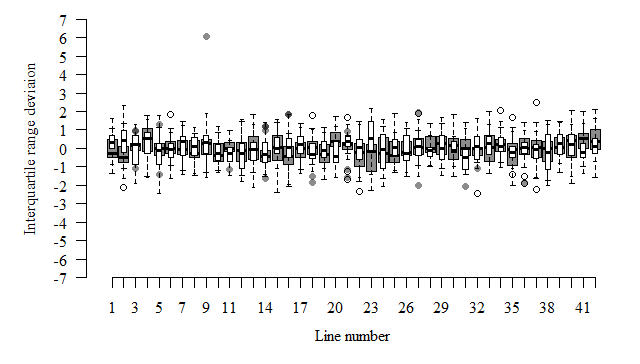
\includegraphics[width=1\textwidth]{Supp/Chp4_DNA/MultiBreedingVals.png}
\caption[Distribution of breeding values for twenty traits for each of the forty-two MA lines. ]{\textbf{Distribution of breeding values for twenty traits for each of the forty-two MA lines.} Equation \ref{eqn:FitlogOR} was used to estimate best linear unbiased predictors (BLUPs) separately for each trait, for the terminal generation, excluding univariate outliers [for each trait] that exceeded 3.0 standard deviations from the mean. Traits consisted of ten fly wing inter-vein landmark distances and, fly wing centroid size (see Chapter 2 methods); eight log-contrasts of cuticular hydrocarbons (CHCs); and, the log-ratio for fitness (main text, Figure \ref{fig:FitBlups}). To compare values across traits, I determined the interquartile range (IQR) deviations for each breeding value, for a trait, within a treatment. IQR deviations are more robust to detecting extreme outliers, where I considered outliers as anything deviating more than 3 IQR from the median. For each MA line, grey boxes represent estimates from the Large population size treatment (B), and the overlayed, smaller, white boxes represent the distribution of estimates from the Small population size treatments (S). Points represent estimates that are greater than 1.5 times the interquartile range (B, grey dots; S, white dots). }
    \label{fig:DNAsuppBlups}
\end{figure}

\FloatBarrier

\begin{figure}[!b]
    \centering
    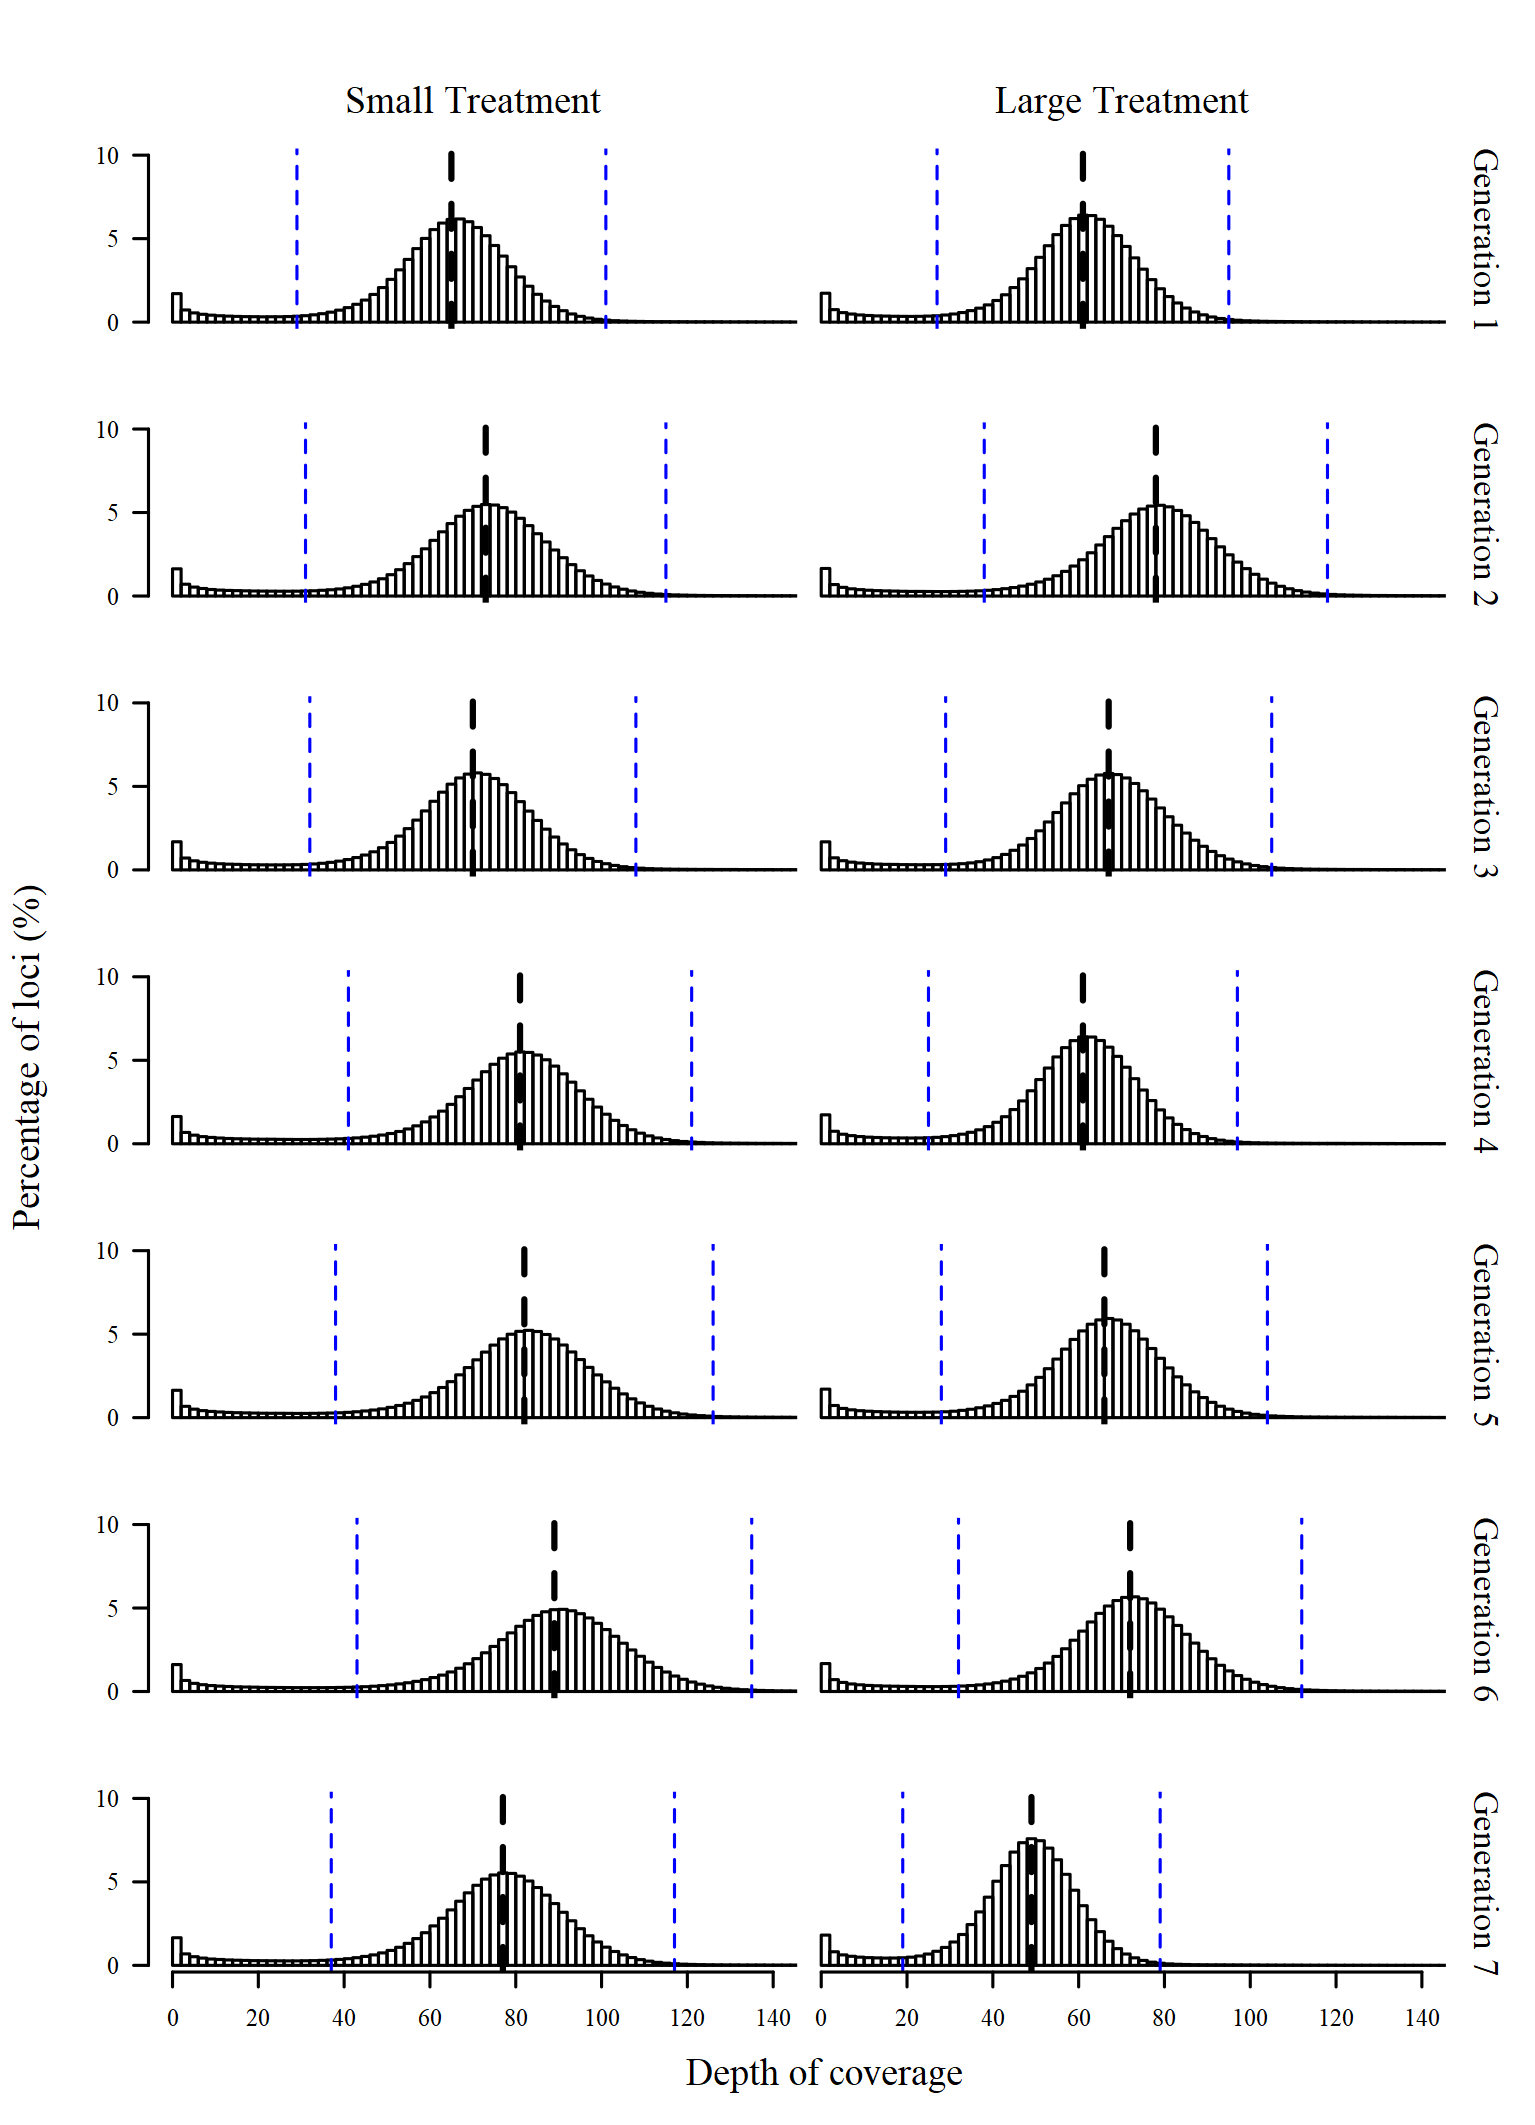
\includegraphics[width=0.85\textwidth]{Supp/Chp4_DNA/Hist22.png}
\caption[Histograms of depth of coverage for the major scaffolds in each pool mapped to the \textit{D. serrata} genome.]{\textbf{Histograms of depth of coverage for the major scaffolds in each pool mapped to the \textit{D. serrata} genome.} The median (vertical black lines) and the depth threshold (median $\pm 2\ \times$~interquartile range, blue dashed lines). The x-axis magnifies the distribution for the range of read depth coverage from 0 to 140, spanning the upper and lower depth thresholds, where right-hand distribution tails range upwards of 100,000.}
    \label{fig:DNAsuppDepthHist}
\end{figure}

\FloatBarrier

\begin{figure}[!htb]
    \centering
    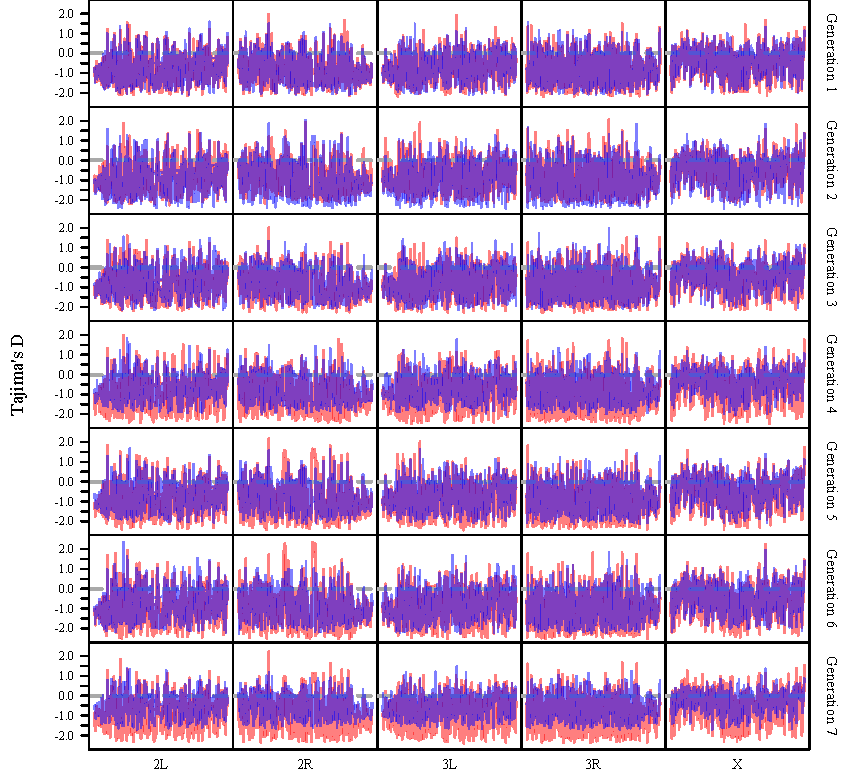
\includegraphics[width=1\textwidth]{Supp/Chp4_DNA/TajimasD_Chrom.pdf}
\caption[Tajima’s D estimates of neutrality along chromosomes arms in non-overlapping 50kbp windows. ]{\textbf{Tajima’s D estimates of neutrality along chromosomes arms in non-overlapping 50kbp windows.} Each panel represents a chromosome arm (x-axis) for each generation (right y-axis). Tajima’s D (left y-axis) was estimated for each treatment separately (S treatment, red; L treatment, blue), where there is large overlap between treatment estimate values (purple). The horizontal grey dash line at zero is the neutral expectation, indicating that the number of segregating sites is equivalent to the number of intermediate-frequency sites. For comparison, I excluded 56 (2\%) of windows that had poor coverage ($< 60\%$ did not meet minimum coverage threshold) that could not be estimated across all pools.}
    \label{fig:DNAsuppTajD}
\end{figure}

\FloatBarrier

\begin{figure}[!htb]
    \centering
    \includegraphics[width=0.85\textwidth]{Supp/Chp4_DNA/2022.20.05_TemporalDiffs.pdf}
\caption[The relationship between the maximum absolute focal allele ($p$) change across a single generation against the temporal change in focal allele ($p$) frequencies.]{\textbf{The relationship between the maximum absolute focal allele ($p$) change across a single generation against the temporal change in focal allele ($p$) frequencies.} Temporal allele frequency differences were determined using the average allele frequency of the two terminal generations (6 and 7) minus the average allele frequency of the two initial generations (1 and 2), where the absolute difference is plotted (x-axis). Deterministic allele frequency change should result in consistent divergence in allele frequencies overtime; however, several loci have large allele frequency differences ($|p_{ti} - p_{ti-1}| > 0.6$; y-axis) across a single generation but this change does not persist through time (i.e., $|$terminal $p$ – initial $p| < 0.55$; x-axis). Further investigation (results not shown) revealed patterns of poor sampling, and these loci were removed from further analyses. }
    \label{fig:DNAsuppBouncyP}
\end{figure}
\vspace{-2cm}
\FloatBarrier
\begin{figure}[!ht]
    \centering
    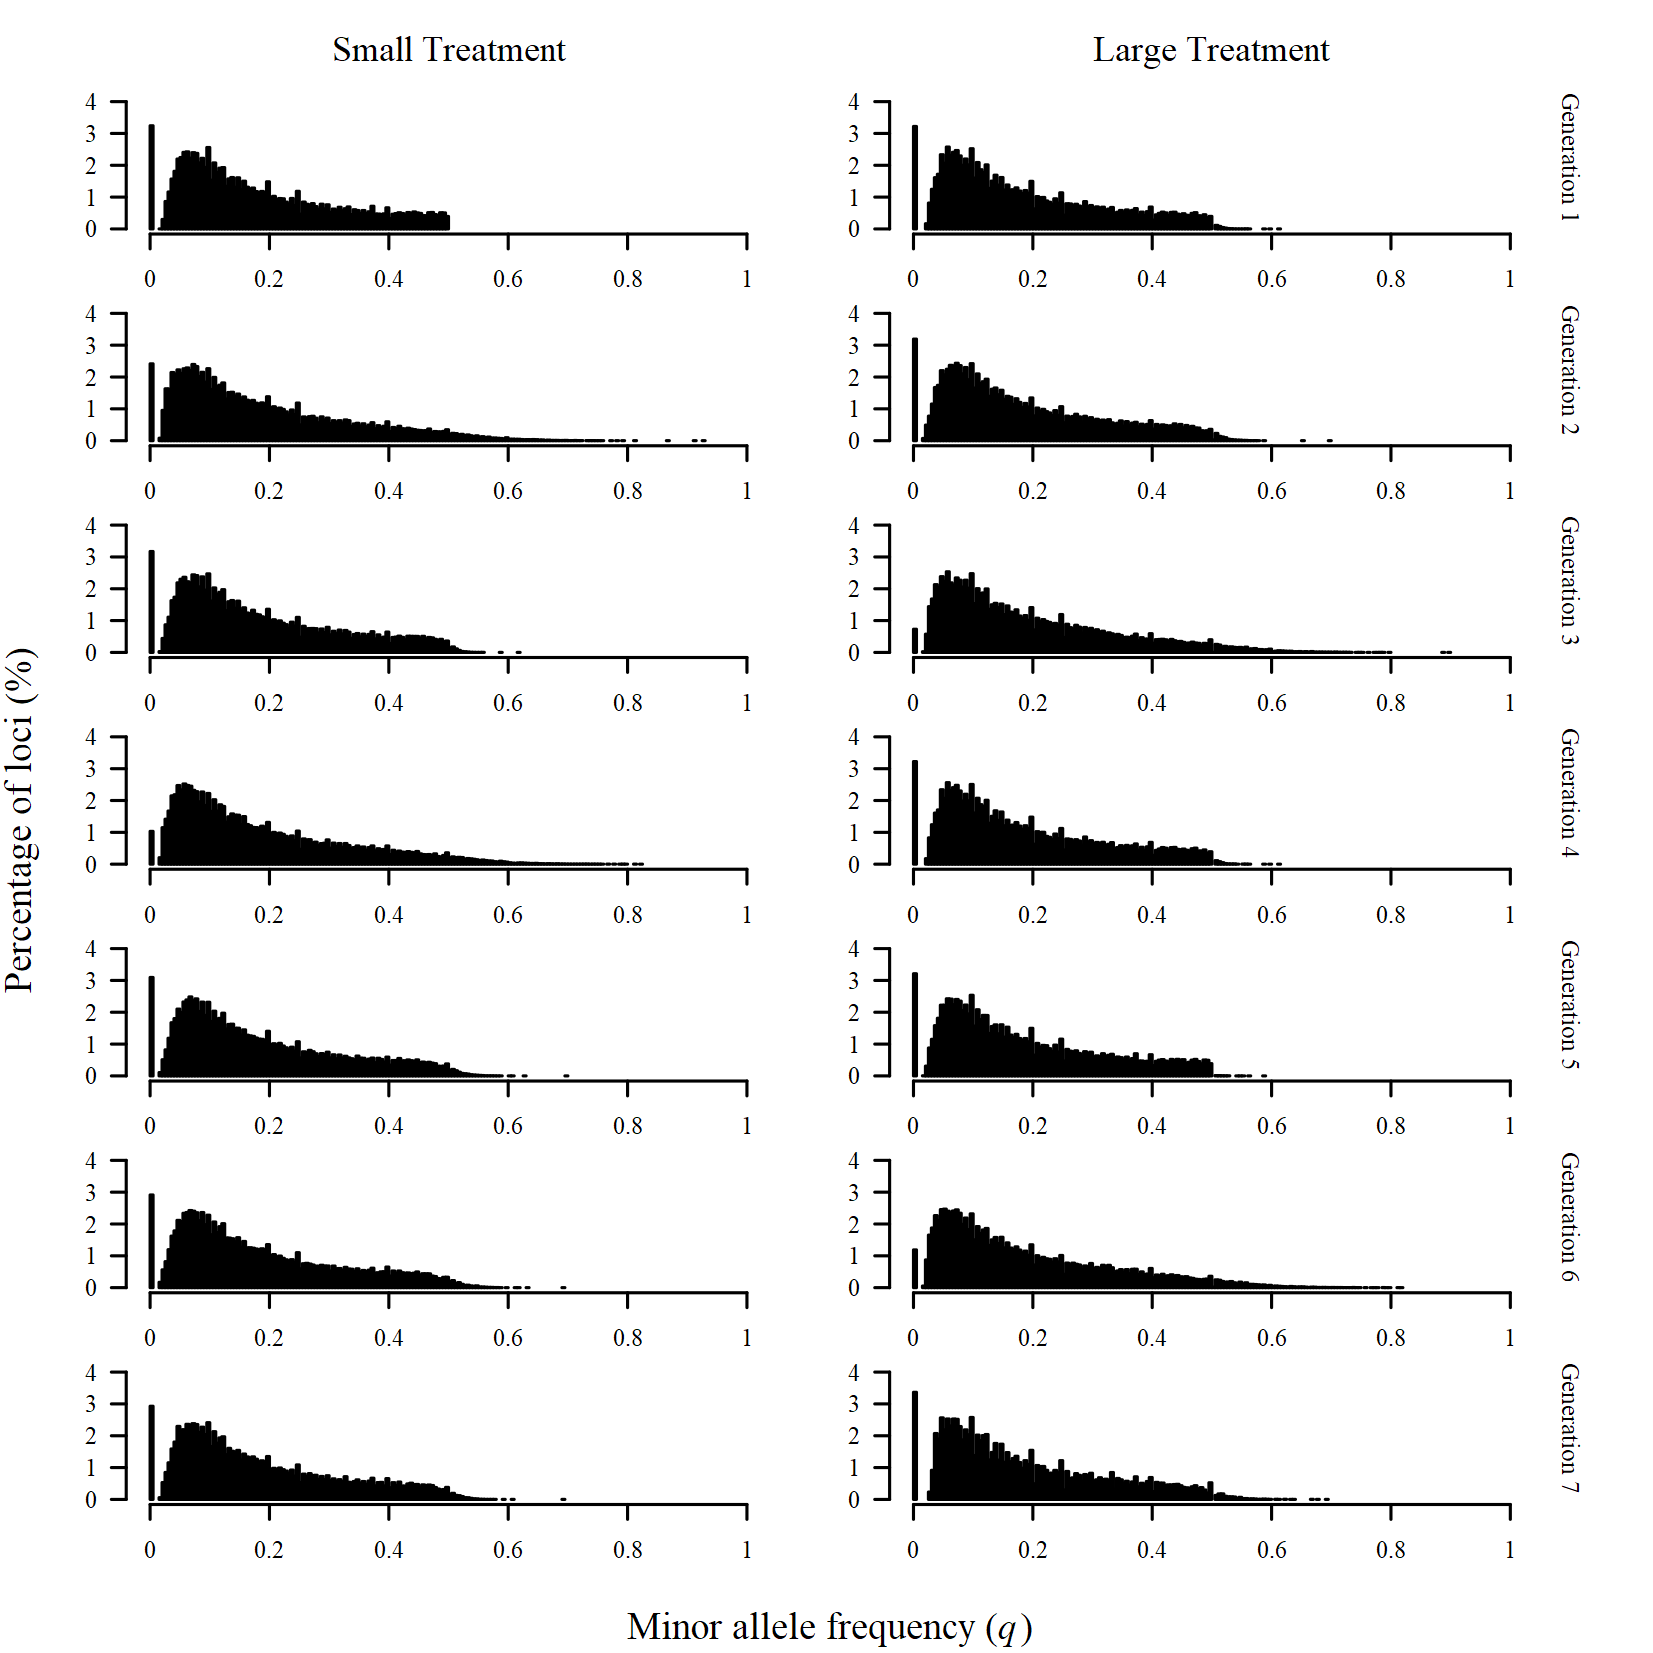
\includegraphics[width=0.7\textwidth]{Supp/Chp4_DNA/MAF_trtxgen_22.png}
\caption[The derived (minor) allele frequency, q, spectrum for SNPs within each treatment for each of the seven generations. ]{\textbf{The derived (minor) allele frequency, $q$, spectrum for SNPs within each treatment for each of the seven generations. } }
    \label{fig:DNAsuppSiteFreqMAF}
\end{figure}

\begin{figure}[!h]
    \centering
    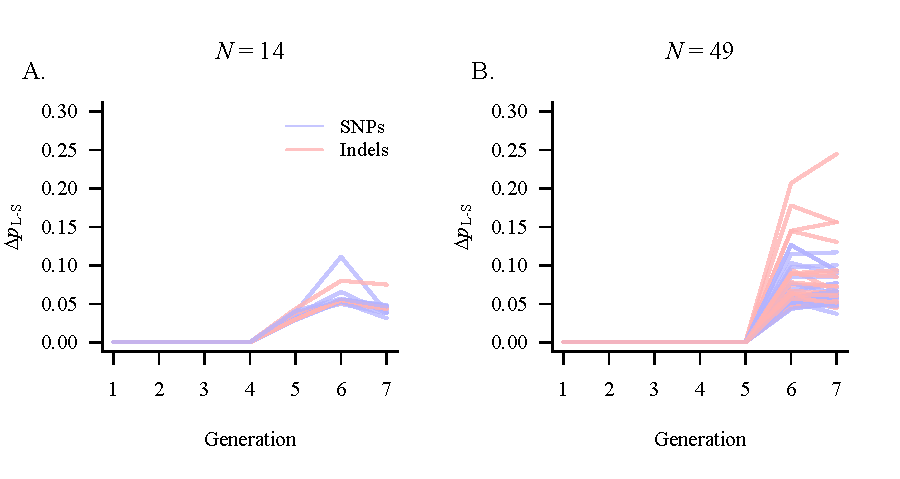
\includegraphics[width=0.75\textwidth]{Supp/Chp4_DNA/TwoInvariants.pdf}
    \vspace{-0.4cm}
\caption[Focal allele frequency difference ($\Delta p_{L-S}$) across time for loci that had a fixed ancestral allele in the large population treatment but had a derived allele arise in the small population treatment.]{\textbf{Focal allele frequency difference ($\Delta p_{L-S}$) across time for loci that had a fixed ancestral allele in the large population treatment but had a derived allele arise in the small population treatment.} Sixty-three loci were screened as novel mutations arising and segregating in the final generations of the experiment. Fourteen loci were distinct in sharing a minor allele that arose after the fourth generation (A), and the remainder of loci had a minor allele arise after the fifth generation (B). Both SNPs (blue lines) and indels (red lines) were considered.}
    \label{fig:DNAsuppInvaraint}
\end{figure}


\FloatBarrier
\begin{figure}[!htb]
    \centering
    \includegraphics[width=0.85\textwidth]{Supp/Chp4_DNA/2023_Coverage6vs7.pdf}
\caption[Coverage of loci in the sixth generation against coverage in the seventh generation, plotting the small (A and C) and large (B and D) population treatments separately. ]{\textbf{Coverage of loci in the sixth generation against coverage in the seventh generation, plotting the small (A and C) and large (B and D) population treatments separately.} Comparisons were made for all loci (top panels) and the 12,352 loci that were outliers for $F_{ST}$ and $\Delta p$ (bottom panels). In C and D, the 248 outliers that were detected across both terminal generations are represented in blue and the corresponding Spearman’s correlation between the coverage in the sixth and seventh generation is on the right plot border in blue.  }
    \label{fig:DNAsuppDepthHist}
\end{figure}

\FloatBarrier

%======Main Eigentensor Eigenvector Loadings========
\begin{table}[!htbp]
\renewcommand{\arraystretch}{1.2}
\begin{center}
\caption[Qualimap sample statistics for sequence alignment for the fourteen pooled populations against the \textit{D. serrata} genome.]{\textbf{Qualimap sample statistics for sequence alignment for the fourteen pooled populations against the \textit{Drosophila serrata} genome.}}
\label{tab:DNAsuppQualimap}
\begin{tabular}{ccS[table-format=2.2]S[table-format=4.2]S[table-format=2.2]S[table-format=2.2]c}
\toprule
\textbf{Population} & \textbf{Generation}
& \multicolumn{1}{m{1.7cm}}{\centering \textbf{Coverage \\ means}}
& \multicolumn{1}{m{1.75cm}}{\centering \textbf{Coverage \\ SD} }
& \multicolumn{1}{m{2cm}}{\centering \textbf{GC \\ percentage} }
& \multicolumn{1}{m{2.8cm}}{\centering \textbf{Mapping quality \\ mean }}
& \multicolumn{1}{m{1.6cm}}{\centering \textbf{Insert size \\ median} }\\[1ex]
\midrule
Small	& 1		& 64.53	& 858.07	& 40.41	& 41.73	& 344 \\
		& 2		& 60.80	& 801.13	& 40.41	& 41.58	& 344 \\
		& 3		& 68.86	& 914.66	& 40.42	& 41.79	& 344 \\
		& 4		& 78.66	& 977.47	& 40.34	& 41.23	& 359 \\
		& 5		& 79.93	& 1060.72	& 40.44	& 41.89	& 344 \\
		& 6		& 86.73	& 1142.54	& 40.44	& 41.90	& 345 \\
		& 7		& 75.06	& 1011.12	& 40.42	& 41.89	& 344 \\ [1.5ex]
Large	& 1		& 60.67	& 801.13	& 40.41	& 41.58	& 344 \\
		& 2		& 76.03	& 1019.99	& 40.43	& 41.87	& 343 \\
		& 3		& 66.26	& 915.28	& 40.67	& 41.34	& 347 \\
		& 4		& 60.71	& 801.13	& 40.41	& 41.58	& 344 \\
		& 5		& 65.34	& 858.09	& 40.43	& 41.73	& 344 \\
		& 6		& 69.77	& 850.40	& 40.37	& 41.20	& 358 \\
		& 7		& 48.48	& 637.48	& 40.40	& 41.18	& 343 \\ [1ex]
\bottomrule
\end{tabular}
\end{center}
\end{table}

\begin{table}[!b]
\renewcommand{\arraystretch}{1.3}
\begin{center}
\caption[Statistical support for the effect of population size treatments within a generation on Tajima’s D test for genomic neutrality.]{\textbf{Statistical support for the effect of population size treatments within a generation on Tajima’s D test for genomic neutrality.} Post-hoc pairwise Kruskal-Wallis rank sum tests were used to determine if there were differences in the treatment medians of the 50 kbp non-overlapping window estimates of Tajima’s D within each sampled generation. Each $H$ statistic had one degree of freedom, where the $P$-values were corrected for multiple testing using a 5\% false discovery rate, (5\%~FDR~$P$-value; significant tests in bold).}
\label{tab:DNAsuppKruskalW}
\begin{tabular}{cS[table-format=3.2]cS[table-format=1.3]S[table-format=1.3]}
\toprule
\textbf{Generation}	& \bfseries{$H$} & \textbf{Degrees of freedom}	& \textbf{$P$-{}-value} & \textbf{5\% FDR $P$--value} \\
\midrule
1	& 2.06	& 1	& 0.151	             & 0.151\\
2	& 35.68	& 1	& \textbf{0.000}	& \textbf{0.000}\\
3	& 13.76	& 1	& \textbf{0.000}	& \textbf{0.000}\\
4	& 280.37 &	1	& \textbf{0.000}	& \textbf{0.000}\\
5	& 74.43	& 1 	& \textbf{0.000}	& \textbf{0.000}\\
6	& 68.62	& 1	& \textbf{0.000}	& \textbf{0.000}\\
7	& 426.56 &	1	& \textbf{0.000}	& \textbf{0.000}\\
\bottomrule
\end{tabular}
\end{center}
\end{table}

\begin{table}[!htbp]
\renewcommand{\arraystretch}{1.4}
\begin{center}
\caption[Variant calling using FreeBayes-parallel.]{\textbf{Variant calling using FreeBayes-parallel.} FreeBayes processes aligned sequencing reads from the BAM format and produces a variant call format (VCF) file containing per position variant calls. Parameters were set (as below) to report observed counts of SNPs, indels and non-variant (fixed) regions. FreeBayes-parallel was run separately for each of the 14 ($n$) poolseq samples, and processing was optimised within a parallel framework.}
\label{tab:DNAsuppFreeBayParms}
\begin{tabular}{p{0.31\textwidth}p{0.59\textwidth}}
\toprule
\textbf{Model Parameter}	& \textbf{Description} \\
\midrule
 -{}- region $n$. regions	& Region files specifying 800 regions of equal coverage generated using the supplied \textit{coverage\_to\_regions.py} script for the $n^{th}$ pooled sample. \\
22	& The number of cores used.\\
-{}-fasta-reference dserrata.fasta &	Fasta reference genome file for \textit{Drosophila serrata}.\\
-{}-min-base-quality 20	& Minimum base quality for an allele, set using the Phred score indicating the probability for the allele nucleotide base (Phred score of 20 ~ 99\% accuracy).\\
-{}-min-mapping-quality 20	& Minimum mapping quality removes alignments from analysis if the probability of read alignment to the reference genome is less than 20. \\
-{}-min-alternate-count 2 & The minimum coverage (number of reads) for an alternate allele is 2, as recommended by \citet{Kofl11}.\\
-{}-min-alternate-fraction $q$	& The alternate fraction ($q$) of observations (reads) for the alternate allele was set to zero. For a coverage of 80 (40 diploid females), the lowest possible $q$ is 0.0125. However, coverage was variable where some loci exceeded 80 (and $q$ < 0.0125 became possible). Setting a threshold >0 might bias against detecting alleles in some pools.\\
-{}-min-coverage $i$	& The minimum coverage ($i$) at a locus was calculated per sample, as the median read depth minus twice the interquartile range (Figure \ref{fig:DNAsuppDepthHist}). This minimises the influence of sequencing errors. \\ 
-{}-skip-coverage $j$ & The maximum coverage ($j$) was the upper coverage limit for loci, and was calculated here, per sample, as the median read depth plus twice the interquartile range (Figure \ref{fig:DNAsuppDepthHist}). By setting a maximum coverage length we both avoid repetitive regions and aid with computational demands due to running analyses in parallel.\\
-{}-haplotype-length -1 &	We ensured whole alignments were considered for variant calling by removing the minimum haplotype length restriction (value of 1 – indicates parameter is not used).\\
-{}-report-monomorphic &	Reports the read depth for both variant and non-variant loci.\\
-{}-pooled-continuous &	Output all alleles which pass input filters.\\
-{}-bam $n$. bam	& The $n^{th}$ pooled sample bam file.\\
\bottomrule
\end{tabular}
\end{center}
\end{table}

\begin{table}[!b]
\renewcommand{\arraystretch}{0.94}
\begin{center}
\tiny
\caption[Summary of the 63 loci invariant in the large population treatment but segregating within the small population treatment.]{\textbf{Summary of the 63 loci invariant in the large population treatment but segregating within the small population treatment.} Chromosome (Chr.), Scaffold and Position provide the locus position where Reference allele is the reference genome base assembled by \citet{Alle17B}. The Focal allele (MA ancestral), defined as the major allele ($p$) in the first generation of the small population, was fixed in the large population treatment. The variant (Minor, derived, $q$) allele was only detected in the small treatment, categorised as either an Indel or SNP (TYPE) with reference to the focal allele. Focal [derived] alleles identical to the ancestral reference base are italicised and highlighted in red [blue]; non-italicised variants are novel. Using SNPEff \citep{Cing12}, loci were localised to either an intergenic or exonic Region in the annotated \textit{Drosophila serrata} genome. Maximum minor allele frequency (MAF) and minor allele coverage. Metrics of treatment divergence: Spearman's Rank coefficient for focal allele frequency difference ($\rho\Delta p_{L-S}$) and pairwise $F_{ST}$ for generation six are defined in the Main Methods. Asterisks after $F_{ST}$ values indicate locus was present in the outlier analyses (Main Methods; Figure \ref{fig:FitFstNdeltapDists}).}
\label{tab:DNAsupp63Invaraint}
\begin{tabular}{ccS[table-format=8.0]ccccccS[table-format=2.0]S[table-format=1.2]S[table-format=1.3]}
\toprule
\textbf{Chr.} & \textbf{Scaffold} &
\textbf{Position} & 
\multicolumn{1}{m{0.8cm}}{\centering \textbf{Reference\\Allele}} &
\multicolumn{1}{m{1.7cm}}{\centering \textbf{Focal Allele\\(major, $p$)}} &
\multicolumn{1}{m{1.2cm}}{\centering \textbf{Minor Allele\\(minor, $q$)}} & 
\textbf{Type} & \textbf{Region} &
\multicolumn{1}{m{0.5cm}}{\centering \textbf{Max.\\MAF}} &
\multicolumn{1}{m{1.1cm}}{\centering \textbf{Maximum\\minor allele\\coverage}} &
\multicolumn{1}{m{1.1cm}}{\centering \textbf{Spearman's\\rank\\coefficient}} &
\multicolumn{1}{m{1.2cm}}{\centering \textbf{Generation 6  \\ $F_{ST}$}}\\
\midrule
 2L& SCA8VGG\_542; & 1234066 & T & \textcolor{red}{\textit{T}} & G & SNP & Exonic & 0.11 & 5 & 0.84 & 0.06\\
 & HRSCAF=776 & 1639640 & A & AT & \textcolor{blue}{\textit{A}} & SNP & Exonic & 0.10 & 8 & 0.80 & 0.05\\
 &  & 7384086 & T & TA & \textcolor{blue}{\textit{T}} & SNP & Exonic & 0.07 & 4 & 0.80 & 0.03\\
 &  & 7461873 & C & CA & \textcolor{blue}{\textit{C}} & SNP & Exonic & 0.05 & 5 & 0.76 & 0.03\\
 &  & 8545894 & C & CT & \textcolor{blue}{\textit{C}} & SNP & Exonic & 0.06 & 5 & 0.80 & 0.02\\
 &  & 9145300 & A & AT & \textcolor{blue}{\textit{A}} & SNP & Intergenic & 0.05 & 4 & 0.76 & 0.03\\
 &  & 5875146 & C & CT & \textcolor{blue}{\textit{C}} & SNP & Intergenic & 0.06 & 4 & 0.80 & 0.03\\
 &  & 10662091 & G & GA & \textcolor{blue}{\textit{G}} & SNP & Intergenic & 0.08 & 5 & 0.80 & 0.03\\
 &  & 11873033 & C & \textcolor{red}{\textit{C}} & T & SNP & Intergenic & 0.05 & 3 & 0.80 & 0.02\\
 &  & 12260645 & C & CCTTTT & \textcolor{blue}{\textit{C}} & Indel & Exonic & 0.09 & 5 & 0.76 & 0.05\\
 &  & 13210226 & A & AT & \textcolor{blue}{\textit{A}} & SNP & Intergenic & 0.09 & 5 & 0.80 & 0.04\\
 &  & 14708933 & C & CT & T & SNP & Intergenic & 0.05 & 3 & 0.80 & 0.02\\
 &  & 15844684 & T & TAC & \textcolor{blue}{\textit{T}} & Indel & Exonic & 0.24 & 12 & 0.80 & 0.12*\\
 &  & 16408575 & G & \textcolor{red}{\textit{G}} & T & SNP & Intergenic & 0.08 & 3 & 0.80 & 0.04\\
 & SCA8VGG\_718; & 4557345 & T & TA & \textcolor{blue}{\textit{T}} & SNP & Intergenic & 0.06 & 5 & 0.80 & 0.02\\
 & HRSCAF=1046 & 7794908 & A & ATT & \textcolor{blue}{\textit{A}} & Indel & Exonic & 0.09 & 8 & 0.76 & 0.05\\
 &  & 8347816 & G & GC & \textcolor{blue}{\textit{G}} & SNP & Exonic & 0.06 & 5 & 0.80 & 0.03\\
 &  & 8539578 & A & AT & \textcolor{blue}{\textit{A}} & SNP & Intergenic & 0.06 & 5 & 0.80 & 0.03\\
 \midrule
 2R & SCA8VGG\_785; & 1666529 & G & GA & \textcolor{blue}{\textit{G}} & SNP & Intergenic & 0.05 & 4 & 0.76 & 0.03\\
 & HRSCAF=1140 & 9693364 & C & CCTT & T & Indel & Intergenic & 0.06 & 4 & 0.76 & 0.03\\
 &  & 14395585 & A & AAATAT & \textcolor{blue}{\textit{A}} & Indel & Intergenic & 0.06 & 5 & 0.76 & 0.03\\
 &  & 22443906 & C & CACACCCAT & \textcolor{blue}{\textit{C}} & Indel & Exonic & 0.09 & 6 & 0.80 & 0.05\\
 &  & 24888644 & G & GA & \textcolor{blue}{\textit{G}} & SNP & Exonic & 0.05 & 3 & 0.80 & 0.02\\
 \midrule
3L & SCA8VGG\_628; & 5833643 & G & GA & A & SNP & Exonic & 0.06 & 3 & 0.80 & 0.03\\
 & HRSCAF=890 & 7952621 & A & AT & \textcolor{blue}{\textit{A}} & SNP & Exonic & 0.12 & 10 & 0.80 & 0.06\\
 &  & 14360368 & C & CA & A & SNP & Intergenic & 0.05 & 4 & 0.87 & 0.03\\
 &  & 23440216 & G & \textcolor{red}{\textit{G}} & A & SNP & Intergenic & 0.06 & 4 & 0.87 & 0.03\\
 &  & 23440217 & G & A & \textcolor{blue}{\textit{G}} & SNP & Intergenic & 0.05 & 4 & 0.87 & 0.03\\
 &  & 23440228 & C &\textcolor{red}{\textit{C}} & T & SNP & Intergenic & 0.06 & 4 & 0.87 & 0.03\\
 &  & 23440245 & T &\textcolor{red}{\textit{T}} & TA & Indel & Intergenic & 0.05 & 4 & 0.87 & 0.03\\
 &  & 23440246 & C &\textcolor{red}{\textit{C}} & CAAA & Indel & Intergenic & 0.05 & 4 & 0.87 & 0.03\\
 &  & 23440248 & C &\textcolor{red}{\textit{C}} & CT & Indel & Intergenic & 0.05 & 4 & 0.87 & 0.03\\
 &  & 24054133 & T & A & \textcolor{blue}{\textit{T}} & SNP & Intergenic & 0.1 & 7 & 0.76 & 0.05\\
 &  & 28892440 & C & CA & \textcolor{blue}{\textit{C}} & SNP & Exonic & 0.05 & 5 & 0.76 & 0.03\\
 &  & 29254069 & G & GGTT & \textcolor{blue}{\textit{G}} & Indel & Exonic & 0.08 & 6 & 0.76 & 0.04\\
 \midrule
 3R & SCA8VGG\_76; & 814769 & A & ATTT & \textcolor{blue}{\textit{A}} & Indel & Exonic & 0.06 & 5 & 0.76 & 0.03\\
 & HRSCAF=120 & 2659155 & C & T & A & SNP & Intergenic & 0.06 & 3 & 0.87 & 0.03\\
 &  & 16381559 & CT & C & \textcolor{blue}{\textit{CT}} & Indel & Intergenic & 0.09 & 7 & 0.80 & 0.05\\
 &  & 17422635 & C & CT & T & SNP & Exonic & 0.06 & 4 & 0.80 & 0.03\\
 &  & 17882837 & C & T & \textcolor{blue}{\textit{C}} & SNP & Exonic & 0.13 & 11 & 0.76 & 0.07*\\
 &  & 17882838 & T & C & \textcolor{blue}{\textit{T}} & SNP & Exonic & 0.13 & 11 & 0.76 & 0.07*\\
 &  & 20830093 & T & TTTTGCTTTGC & C & Indel & Intergenic & 0.05 & 3 & 0.80 & 0.02\\
 &  & 21122946 & A & AT & \textcolor{blue}{\textit{A}} & SNP & Exonic & 0.06 & 5 & 0.76 & 0.03\\
 &  & 24407217 & GCAG & G & \textcolor{blue}{\textit{GCAG}} & Indel & Exonic & 0.07 & 4 & 0.80 & 0.03\\
 &  & 26267574 & TA & T & \textcolor{blue}{\textit{TA}} & Indel & Exonic & 0.07 & 6 & 0.76 & 0.03\\
 &  & 26373577 & AAT & \textcolor{red}{\textit{AAT}} & A & Indel & Intergenic & 0.08 & 4 & 0.87 & 0.04\\
 &  & 35443451 & C & \textcolor{red}{\textit{C}} & A & SNP & Intergenic & 0.07 & 3 & 0.80 & 0.03\\
 \midrule
 X & SCA8VGG\_594; & 5513872 & T & \textcolor{red}{\textit{T}} & A & SNP & Intergenic & 0.05 & 3 & 0.87 & 0.03\\
 & HRSCAF=845 & 7843237 & A & AGGTAGGAAG & \textcolor{blue}{\textit{A}} & Indel & Exonic & 0.14 & 11 & 0.76 & 0.08*\\
 &  & 8365245 & G & \textcolor{red}{\textit{G}} & A & SNP & Exonic & 0.06 & 3 & 0.80 & 0.03\\
 &  & 9151570 & TGAG & T & TAG & Indel & Exonic & 0.05 & 3 & 0.87 & 0.03\\
 &  & 10260205 & C &\textcolor{red}{\textit{C}} & A & SNP & Intergenic & 0.07 & 3 & 0.80 & 0.03\\
 &  & 10260225 & G &\textcolor{red}{\textit{G}} & T & SNP & Intergenic & 0.05 & 3 & 0.80 & 0.02\\
 &  & 14676663 & A &\textcolor{red}{\textit{A}} & C & SNP & Exonic & 0.06 & 3 & 0.80 & 0.02\\
 &  & 16995279 & G & A & \textcolor{blue}{\textit{G}} & SNP & Intergenic & 0.06 & 6 & 0.76 & 0.03\\
 &  & 17885746 & CA & C & \textcolor{blue}{\textit{CA}} & Indel & Intergenic & 0.07 & 6 & 0.76 & 0.04\\
 &  & 18673610 & C & CAAACCCAATAA & \textcolor{blue}{\textit{C}} & Indel & Exonic & 0.16 & 10 & 0.80 & 0.08*\\
 &  & 24454337 & T & C & \textcolor{blue}{\textit{T}} & SNP & Intergenic & 0.07 & 4 & 0.87 & 0.03\\
 &  & 26336051 & C & CA & A & SNP & Exonic & 0.05 & 3 & 0.80 & 0.02\\
 &  & 26891723 & C & T & \textcolor{blue}{\textit{C}} & SNP & Intergenic & 0.05 & 3 & 0.87 & 0.03\\
 &  & 27919844 & A & ATTC & \textcolor{blue}{\textit{A}} & Indel & Intergenic & 0.18 & 16 & 0.76 & 0.10*\\
 &  & 28556020 & C & CA & \textcolor{blue}{\textit{C}} & SNP & Exonic & 0.08 & 7 & 0.76 & 0.04\\
 &  & 28860275 & C & CA & \textcolor{blue}{\textit{C}} & SNP & Exonic & 0.05 & 4 & 0.80 & 0.02\\
\bottomrule
\end{tabular}
\end{center}
\end{table}

\begin{table}[!b]
\renewcommand{\arraystretch}{1}
\begin{center}
\small
\caption[SnpEff (v5.1) annotation for the 248 outlier loci.]{\textbf{SnpEff (v5.1) annotation for the 248 outlier loci.} There were 511 unique annotations, with some variants having multiple annotations (median number per loci = 2 and maximum =~5). Eleven categories of putative loci effect were further classified by functional impact (high, moderate, low and modifier). }
\label{tab:DNAsuppSnpEff}
\begin{tabular}{lcS[table-format=3.0]S[table-format=2.1]}
\toprule
\textbf{SnpEff Annotation} & \textbf{Functional Impact} &
\textbf{Number of loci} & \textbf{Percentage}\\
\midrule
3\_prime\_UTR\_variant&modifier&1&0.2\%\\
5\_prime\_UTR\_variant&modifier&1&0.2\%\\
downstream\_gene\_variant&modifier&67&13.1\%\\
intergenic\_region&modifier&130&25.4\%\\
intragenic\_variant&modifier&11&2.2\%\\
intron\_variant&modifier&108&21.1\%\\
missense\_variant&moderate&4&0.8\%\\
non\_coding\_transcript\_exon\_variant&modifier&4&0.8\%\\
non\_coding\_transcript\_variant&modifier&108&21.1\%\\
synonymous\_variant&low&1&0.2\%\\
upstream\_gene\_variant&modifier&76&14.9\%\\
\bottomrule
\end{tabular}
\end{center}
\end{table}

\newpage
\FloatBarrier
\begin{table}[!b]
\renewcommand{\arraystretch}{1.2}
\begin{center}
\small
\caption[Gene enrichment analysis of gene ontology (GO) terms of the \textit{Drosophila melanogaster} orthologs for the candidate outliers.]{Gene enrichment analysis of gene ontology (GO) terms of the \textit{Drosophila melanogaster} orthologs for the candidate outliers. Fifty-eight unique \textit{D. melanogaster} orthologs were identified for the 53 candidate \textit{Drosophila serrata} Line 9 outlier loci (Table~\ref{tab:Fit53outliers}). GO terms consist of three categories (Type): biological processes (BP), molecular function (MF) and cellular function (CF). The number of Sample loci were tested against the Background number of genes containing the GO term and were assess using a Fisher’s Exact test and corrected using a 0.05 False Discovery Rate (FDR). Bold GO terms represent supergroups and are followed by the corresponding subgroup GO terms.}
\label{tab:DNAsuppGOterms}
\tiny
\begin{tabular}{clS[table-format=4.0]S[table-format=2.0]S[table-format=2.2]ccc}
\toprule
\textbf{Type} &\textbf{GO Term} &\textbf{Background} &\textbf{Sample} &\textbf{Expected} &\textbf{fold Enrichment} &\textbf{$P-$value} &\textbf{FDR $P-$value}\\
\midrule
BP & \textbf{mitochondrial ADP transmembrane transport (GO:0140021)} & 2 & 2 & 0.01 & $> 100$ & 5.36E-05 & 1.60E-02 \\
 & cellular process (GO:0009987) & 7238 & 34 & 22.00 & $1.55$ & 1.56E-04 & 2.38E-02 \\
 & purine-containing compound transmembrane transport (GO:0072530) & 2 & 2 & 0.01 & $> 100$ & 5.36E-05 & 1.49E-02 \\
 & nucleotide transmembrane transport (GO:1901679) & 3 & 2 & 0.01 & $> 100$ & 8.91E-05 & 1.74E-02 \\
 & nucleotide transport (GO:0006862) & 7 & 2 & 0.02 & $94.02$ & 3.18E-04 & 3.94E-02 \\
 & ADP transport (GO:0015866) & 2 & 2 & 0.01 & $> 100$ & 5.36E-05 & 1.67E-02 \\
 & purine ribonucleotide transport (GO:0015868) & 5 & 2 & 0.02 & $> 100$ & 1.86E-04 & 2.74E-02 \\
 & purine nucleotide transport (GO:0015865) & 5 & 2 & 0.02 & $> 100$ & 1.86E-04 & 2.69E-02 \\
 & adenine nucleotide transport (GO:0051503) & 4 & 2 & 0.01 & $> 100$ & 1.33E-04 & 2.21E-02 \\[1.5ex]
 & \textbf{mitochondrial ATP transmembrane transport (GO:1990544)} & 2 & 2 & 0.01 & $> 100$ & 5.36E-05 & 1.55E-02 \\
 & ATP transport (GO:0015867) & 2 & 2 & 0.01 & $> 100$ & 5.36E-05 & 1.74E-02 \\[1.5ex]
 & \textbf{negative regulation of mitochondrial outer membrane permeabilization}& 3 & 2 & 0.01 & $> 100$ & 8.91E-05 & 1.83E-02 \\ [-1ex]
 &\textbf{involved in apoptotic signalling pathway (GO:1901029)} &  &  &  & &  &  \\
 & regulation of cellular process (GO:0050794) & 3690 & 23 & 11.21 & $2.05$ & 1.45E-04 & 2.27E-02 \\
 & regulation of biological process (GO:0050789) & 4030 & 27 & 12.25 & $2.2$ & 3.10E-06 & 8.05E-03 \\
 & biological regulation (GO:0065007) & 4471 & 27 & 13.59 & $1.99$ & 3.76E-05 & 1.46E-02 \\
 & negative regulation of programmed cell death (GO:0043069) & 117 & 4 & 0.36 & $11.25$ & 4.78E-04 & 4.90E-02 \\
 & negative regulation of mitochondrial membrane permeability (GO:0035795) & 3 & 2 & 0.01 & $> 100$ & 8.91E-05 & 1.88E-02 \\
 & regulation of mitochondrial membrane permeability (GO:0046902) & 6 & 2 & 0.02 & $> 100$ & 2.48E-04 & 3.22E-02 \\
 & regulation of membrane permeability (GO:0090559) & 6 & 2 & 0.02 & $> 100$ & 2.48E-04 & 3.17E-02 \\
 & cellular component organization (GO:0016043) & 2644 & 18 & 8.03 & $2.24$ & 4.95E-04 & 4.94E-02 \\
 & negative regulation of membrane permeability (GO:1905709) & 3 & 2 & 0.01 & $> 100$ & 8.91E-05 & 1.69E-02 \\
 & regulation of mitochondrial outer membrane permeabilization involved in & 3 & 2 & 0.01 & $> 100$ & 8.91E-05 & 1.78E-02 \\[-1ex]
 & apoptotic signalling pathway (GO:1901028) &  &  &  & &  &  \\[1.5ex]
 & \textbf{positive regulation of stress fibre assembly (GO:0051496)} & 6 & 2 & 0.02 & $> 100$ & 2.48E-04 & 3.12E-02 \\
 & positive regulation of actin filament bundle assembly (GO:0032233) & 8 & 2 & 0.02 & $82.27$ & 3.97E-04 & 4.48E-02 \\
 & positive regulation of supramolecular fibre organization (GO:1902905) & 44 & 3 & 0.13 & $22.44$ & 3.82E-04 & 4.51E-02 \\
 & positive regulation of cytoskeleton organization (GO:0051495) & 47 & 3 & 0.14 & $21$ & 4.59E-04 & 4.90E-02 \\[1.5ex]
 & \textbf{tracheal pit formation in open tracheal system (GO:0035202)} & 10 & 3 & 0.03 & $98.72$ & 7.24E-06 & 7.05E-03 \\
 & system development (GO:0048731) & 1339 & 15 & 4.07 & $3.69$ & 5.03E-06 & 9.79E-03 \\
 & anatomical structure development (GO:0048856) & 2531 & 18 & 7.69 & $2.34$ & 2.10E-04 & 2.92E-02 \\
 & multicellular organism development (GO:0007275) & 2125 & 18 & 6.46 & $2.79$ & 1.99E-05 & 9.12E-03 \\
 & multicellular organismal process (GO:0032501) & 3331 & 22 & 10.12 & $2.17$ & 8.26E-05 & 1.84E-02 \\
 & anatomical structure morphogenesis (GO:0009653) & 1466 & 14 & 4.45 & $3.14$ & 6.93E-05 & 1.80E-02 \\[1.5ex]
 & \textbf{lymph gland plasmatocyte differentiation (GO:0035169)} & 7 & 2 & 0.02 & $94.02$ & 3.18E-04 & 3.87E-02 \\
 & post-embryonic animal organ development (GO:0048569) & 462 & 7 & 1.40 & $4.99$ & 4.69E-04 & 4.93E-02 \\
 & animal organ development (GO:0048513) & 1162 & 14 & 3.53 & $3.96$ & 5.07E-06 & 7.90E-03 \\[1.5ex]
 & \textbf{integrin-mediated signalling pathway (GO:0007229)} & 11 & 3 & 0.03 & $89.75$ & 9.20E-06 & 7.96E-03 \\
 & cell surface receptor signalling pathway (GO:0007166) & 311 & 7 & 0.95 & $7.41$ & 4.23E-05 & 1.57E-02 \\
 & signal transduction (GO:0007165) & 1000 & 12 & 3.04 & $3.95$ & 3.05E-05 & 1.25E-02 \\
 & signalling (GO:0023052) & 1198 & 14 & 3.64 & $3.85$ & 7.21E-06 & 8.02E-03 \\
 & cell communication (GO:0007154) & 1268 & 14 & 3.85 & $3.63$ & 1.38E-05 & 9.76E-03 \\
 & cellular response to stimulus (GO:0051716) & 1496 & 14 & 4.55 & $3.08$ & 8.63E-05 & 1.87E-02 \\
 & response to stimulus (GO:0050896) & 2530 & 20 & 7.69 & $2.6$ & 1.45E-05 & 8.06E-03 \\[1.5ex]
 & \textbf{cell-matrix adhesion (GO:0007160)} & 17 & 4 & 0.05 & $77.43$ & 4.20E-07 & 3.27E-03 \\
 & cell-substrate adhesion (GO:0031589) & 24 & 4 & 0.07 & $54.85$ & 1.41E-06 & 5.51E-03 \\
 & cell adhesion (GO:0007155) & 179 & 6 & 0.54 & $11.03$ & 1.83E-05 & 8.92E-03 \\[1.5ex]
 & \textbf{cardiac muscle tissue development (GO:0048738)} & 9 & 2 & 0.03 & $73.13$ & 4.84E-04 & 4.90E-02 \\
 & tissue development (GO:0009888) & 1005 & 13 & 3.05 & $4.26$ & 5.73E-06 & 7.44E-03 \\[1.5ex]
 & \textbf{regulation of wound healing (GO:0061041)} & 17 & 3 & 0.05 & $58.07$ & 2.84E-05 & 1.23E-02 \\
 & regulation of response to wounding (GO:1903034) & 33 & 3 & 0.10 & $29.92$ & 1.72E-04 & 2.58E-02 \\[1.5ex]
 & \textbf{fibroblast growth factor receptor signalling pathway (GO:0008543)} & 25 & 3 & 0.08 & $39.49$ & 8.04E-05 & 1.96E-02 \\
 & cellular response to fibroblast growth factor stimulus (GO:0044344) & 25 & 3 & 0.08 & $39.49$ & 8.04E-05 & 1.90E-02 \\
 & cellular response to growth factor stimulus (GO:0071363) & 45 & 4 & 0.14 & $29.25$ & 1.40E-05 & 9.07E-03 \\
 & response to chemical (GO:0042221) & 1093 & 13 & 3.32 & $3.91$ & 1.41E-05 & 8.46E-03 \\
 & response to growth factor (GO:0070848) & 46 & 4 & 0.14 & $28.61$ & 1.51E-05 & 7.87E-03 \\
 & cellular response to endogenous stimulus (GO:0071495) & 154 & 5 & 0.47 & $10.68$ & 1.13E-04 & 1.95E-02 \\
 & response to endogenous stimulus (GO:0009719) & 162 & 5 & 0.49 & $10.16$ & 1.42E-04 & 2.30E-02 \\
 & response to fibroblast growth factor (GO:0071774) & 25 & 3 & 0.08 & $39.49$ & 8.04E-05 & 2.02E-02 \\[1.5ex]
 & \textbf{epithelial cell morphogenesis (GO:0003382)} & 31 & 3 & 0.09 & $31.85$ & 1.45E-04 & 2.30E-02 \\
 & cell development (GO:0048468) & 1303 & 12 & 3.96 & $3.03$ & 3.76E-04 & 4.51E-02 \\
 & epithelium development (GO:0060429) & 930 & 10 & 2.83 & $3.54$ & 3.92E-04 & 4.56E-02 \\
 %~~~~~~~~~~~~~~~~~~~~~ GAP ~~~~~~~~~~~~~~~~~~~~~~~~~~~~%
 \bottomrule
 \end{tabular}
\end{center}
\end{table}
\FloatBarrier
 \newpage
 \begin{table}[!b]
\renewcommand{\arraystretch}{1.2}
\begin{center}
\small
\tiny
\begin{tabular}{clS[table-format=4.0]S[table-format=2.0]S[table-format=2.2]ccc}
\toprule
\textbf{Type} &\textbf{GO Term (\textit{cont.})} &\textbf{Background} &\textbf{Sample} &\textbf{Expected} &\textbf{fold Enrichment} &\textbf{$P-$value} &\textbf{FDR $P-$value}\\
\midrule
  %~~~~~~~~~~~~~~~~~~~~~ GAP ~~~~~~~~~~~~~~~~~~~~~~~~~~~~%
 BF & \textbf{compound eye morphogenesis (GO:0001745)} & 276 & 6 & 0.84 & $7.15$ & 1.90E-04 & 2.70E-02 \\
 & compound eye development (GO:0048749) & 346 & 7 & 1.05 & $6.66$ & 8.19E-05 & 1.88E-02 \\
 & eye development (GO:0001654) & 364 & 7 & 1.11 & $6.33$ & 1.12E-04 & 2.07E-02 \\
 & sensory organ development (GO:0007423) & 456 & 7 & 1.39 & $5.05$ & 4.34E-04 & 4.83E-02 \\
 & visual system development (GO:0150063) & 364 & 7 & 1.11 & $6.33$ & 1.12E-04 & 2.02E-02 \\
 & sensory system development (GO:0048880) & 364 & 7 & 1.11 & $6.33$ & 1.12E-04 & 1.98E-02 \\
 & eye morphogenesis (GO:0048592) & 285 & 6 & 0.87 & $6.93$ & 2.26E-04 & 2.98E-02 \\
 & sensory organ morphogenesis (GO:0090596) & 285 & 6 & 0.87 & $6.93$ & 2.26E-04 & 3.03E-02 \\
 & animal organ morphogenesis (GO:0009887) & 721 & 10 & 2.19 & $4.56$ & 4.94E-05 & 1.75E-02 \\[1.5ex]
 & \textbf{post-embryonic appendage morphogenesis (GO:0035120)} & 317 & 6 & 0.96 & $6.23$ & 3.95E-04 & 4.52E-02 \\
 & appendage morphogenesis (GO:0035107) & 328 & 6 & 1 & $6.02$ & 4.72E-04 & 4.90E-02 \\
 & appendage development (GO:0048736) & 336 & 7 & 1.02 & $6.86$ & 6.83E-05 & 1.84E-02 \\[1.5ex]
 & \textbf{imaginal disc-derived appendage morphogenesis (GO:0035114)} & 326 & 6 & 0.99 & $6.06$ & 4.57E-04 & 4.95E-02 \\[1.5ex]
 & \textbf{epithelial tube morphogenesis (GO:0060562)} & 460 & 7 & 1.4 & $5.01$ & 4.57E-04 & 5.01E-02 \\
 & morphogenesis of an epithelium (GO:0002009) & 578 & 9 & 1.76 & $5.12$ & 5.24E-05 & 1.77E-02 \\
 & tissue morphogenesis (GO:0048729) & 596 & 10 & 1.81 & $5.52$ & 9.79E-06 & 7.63E-03 \\
 & tube morphogenesis (GO:0035239) & 503 & 8 & 1.53 & $5.23$ & 1.26E-04 & 2.13E-02 \\
 & tube development (GO:0035295) & 696 & 9 & 2.12 & $4.26$ & 2.12E-04 & 2.90E-02 \\
 \midrule
MF & \textbf{phenylalanine 4-monooxygenase activity (GO:0004505)} & 2 & 2 & 0.01 & $> 100$ & 5.36E-05 & 1.43E-02 \\
 & oxidoreductase activity, acting on paired donors, with incorporation or 
 & 3 & 2 & 0.01 & $> 100$ & 8.91E-05 & 1.74E-02 \\[-1ex]
& reduction of molecular oxygen, reduced pteridine as one donor, and  &  &  &  & &  &  \\[-1ex]
& incorporation of one atom of oxygen (GO:0016714)  &  &  &  & &  &  \\[1.5ex]
 & \textbf{ATP:ADP antiporter activity (GO:0005471)} & 2 & 2 & 0.01 & $> 100$ & 5.36E-05 & 1.31E-02 \\
 & ADP transmembrane transporter activity (GO:0015217) & 3 & 2 & 0.01 & $> 100$ & 8.91E-05 & 1.64E-02 \\
 & ion transmembrane transporter activity (GO:0015075) & 484 & 9 & 1.47 & $6.12$ & 1.32E-05 & 9.72E-03 \\
 & ATP transmembrane transporter activity (GO:0005347) & 4 & 2 & 0.01 & $> 100$ & 1.33E-04 & 2.30E-02 \\
 & solute: anion antiporter activity (GO:0140323) & 6 & 2 & 0.02 & $> 100$ & 2.48E-04 & 3.83E-02 \\[1.5ex]
 & \textbf{integrin binding (GO:0005178)} & 19 & 3 & 0.06 & $51.96$ & 3.83E-05 & 1.25E-02 \\
 & cell adhesion molecule binding (GO:0050839) & 74 & 4 & 0.22 & $17.79$ & 8.82E-05 & 1.85E-02 \\[1.5ex]
 & \textbf{DNA-binding transcription factor binding (GO:0140297)} & 70 & 4 & 0.21 & $18.8$ & 7.18E-05 & 1.62E-02 \\[1.5ex]
 & \textbf{DNA-binding transcription activator activity (GO:0001216)} & 95 & 4 & 0.29 & $13.86$ & 2.22E-04 & 3.63E-02 \\[1.5ex]
 & \textbf{ligand-gated ion channel activity (GO:0015276)} & 143 & 6 & 0.43 & $13.81$ & 5.31E-06 & 5.20E-03 \\
 & ion channel activity (GO:0005216) & 259 & 7 & 0.79 & $8.89$ & 1.34E-05 & 7.90E-03 \\
 & inorganic molecular entity transmembrane transporter activity (GO:0015318) & 429 & 7 & 1.3 & $5.37$ & 3.02E-04 & 4.43E-02 \\
 & channel activity (GO:0015267) & 274 & 7 & 0.83 & $8.41$ & 1.92E-05 & 8.04E-03 \\
 & passive transmembrane transporter activity (GO:0022803) & 274 & 7 & 0.83 & $8.41$ & 1.92E-05 & 9.38E-03 \\
 & ligand-gated channel activity (GO:0022834) & 143 & 6 & 0.43 & $13.81$ & 5.31E-06 & 7.80E-03 \\
 & gated channel activity (GO:0022836) & 202 & 7 & 0.61 & $11.4$ & 2.76E-06 & 8.11E-03 \\[1.5ex]
 & \textbf{protein heterodimerization activity (GO:0046982)} & 127 & 5 & 0.39 & $12.96$ & 4.65E-05 & 1.37E-02 \\
 & protein dimerization activity (GO:0046983) & 276 & 7 & 0.84 & $8.35$ & 2.01E-05 & 7.37E-03 \\
 \midrule
CF & \textbf{cell-substrate junction (GO:0030055)} & 44 & 4 & 0.13 & $29.92$ & 1.29E-05 & 5.70E-03 \\
 & anchoring junction (GO:0070161) & 166 & 7 & 0.5 & $13.88$ & 7.79E-07 & 1.04E-03 \\
 & cell junction (GO:0030054) & 466 & 9 & 1.42 & $6.36$ & 9.82E-06 & 6.53E-03 \\
\bottomrule
\end{tabular}
\end{center}
\end{table}


% Type & GO Term (cont.) & Background & Sample & Expected & $fold Enrichment$ & P-value & FDR \\
%  &  &  &  &  & & 0.00E+00 &  P-value \\